% Report.
%
% Copyright (C) 2011  Vladimir Rutsky <altsysrq@gmail.com>
%
% This work is licensed under a Creative Commons Attribution-ShareAlike 3.0 
% Unported License. See <http://creativecommons.org/licenses/by-sa/3.0/> 
% for details.

% TODO: Использовать не "можно оценить", а "оценим".

\documentclass[a4paper,10pt]{article}

% Encoding support.
\usepackage{ucs}
\usepackage[utf8x]{inputenc}
\usepackage[T2A]{fontenc}
\usepackage[russian]{babel}

\usepackage{amsmath, amsthm, amssymb}
\usepackage{commath}

% Indenting first paragraph.
\usepackage{indentfirst}

\usepackage{url}
\usepackage[unicode]{hyperref}

%\usepackage[final]{pdfpages}

\usepackage[pdftex]{graphicx}
\usepackage{subfig}

\usepackage{fancyvrb}
\usepackage{color}
\usepackage{texments}

\newcommand{\HRule}{\rule{\linewidth}{0.5mm}}

% Spaces after commas.
\frenchspacing
% Minimal carrying number of characters,
\righthyphenmin=2

% From K.V.Voroncov Latex in samples, 2005.
\textheight=24cm   % text height
\textwidth=16cm    % text width.
\oddsidemargin=0pt % left side indention
\topmargin=-1.5cm  % top side indention.
\parindent=24pt    % paragraph indent
\parskip=0pt       % distance between paragraphs.
\tolerance=2000
%\flushbottom       % page height aligning
%\hoffset=0cm
%\pagestyle{empty}  % without numeration

\newcommand{\myemail}[1]{%
\href{mailto:#1}{\nolinkurl{#1}}}

\newcommand{\myfunc}[1]{%
\textit{#1}}

\DeclareMathOperator*{\argmax}{\arg\!\max}
\DeclareMathOperator*{\argmin}{\arg\!\min}

\begin{document}

% Title page.
% Report title page.
%
% Copyright (C) 2011  Vladimir Rutsky <altsysrq@gmail.com>
%
% This work is licensed under a Creative Commons Attribution-ShareAlike 3.0 
% Unported License. See <http://creativecommons.org/licenses/by-sa/3.0/> 
% for details.

\begin{titlepage} % начало титульной страницы

\begin{center} % включить выравнивание по центру

\large Санкт-Петербургский государственный политехнический университет\\[5.5cm]
% название института, затем отступ 5,5см

\huge Лабораторная работа~\No\,1\\[0.6cm] % название работы, затем отступ 0,6см
\large по~курсу <<Стохастические модели>>\\[1cm]
\large <<Проверка гипотезы о присутствии закодированного сообщения в наборе кодов>>\\[6cm]
% тема работы, затем отступ 6см

\begin{flushright} % выровнять её содержимое по правому краю
\begin{tabular}{l l}
Студент: & Руцкий~В.\,В.\\
Группа: & 5057/2\\
Преподаватель: & Иванков ~А.\,А.
\end{tabular}
\end{flushright} % конец выравнивания по правому краю

\vfill % заполнить всё доступное ниже пространство

{\large Санкт-Петербург 2011}
\end{center} % закончить выравнивание по центру
\thispagestyle{empty} % не нумеровать страницу
\end{titlepage} % конец титульной страницы

\tableofcontents
\pagebreak

% Content

\section{Постановка задачи}
В данной работе производится анализ лога использования ресурсов сервера
при поступающих заявках на обработку.

В отсутствие заявок уровень использования ресурсов сервера представляет собой 
сумму некоторой постоянной величины загрузки $m$ и случайных отклонений:
$$B(t) = m + \sigma \mathcal{W}(t),$$
где $\mathcal{W}(t)$~--- это винеровский процесс. 
%В дальнейшем вклад этой компоненты будем называть шумом.

Заявки поступают в соответствии с законом распределения Пуассона 
$\mathcal{P}(\lambda)$.
% TODO: Лучше было бы рассматривать $\lambda = \lambda(t)$

При поступлении одной заявки использование ресурсов мгновенно возрастает,
а затем экспоненциально снижается до прежнего уровня.
Увеличение использования ресурсов сервера от одной заявки, 
поступившей в момент времени $t_c$, выражается следующим образом:
$$K_{t_c}(t) = \mathcal{N}(m_c, \sigma_c^2) \cdot \mathrm{I}(t - t_c) \cdot 
    e^{-\lambda_c(t - t_c)},$$
где $\mathrm{I}(x)$~--- фунцкия Хевисайда.%
\footnote{%
Функция Хевисайда: $\mathrm{I}(x) = \left\{
  \begin{array}{rl}
    0, & x < 0 \\
    1, & x \geqslant 0
  \end{array}\right.$.
}
% Экспоненциальное падение можно обосновать с помощью ТМО.
% d K(t) = -\lambda K'(t) dt

В логе использования ресурсов сервера наблюдается общая загрузка сервера:
$$X(t) = B(t) + \sum\limits_{t_c \in T_c}K_{t_c}(t),$$
где $T_c$~--- это моменты времени поступления заявок.

Необходимо по дискретным наблюдениям $x_i$ случайного процесса $X(t)$ 
в моменты времени $t_i, \quad i=1,\ldots,N$
\begin{enumerate}
 \item оценить моменты времени поступления заявок $T_c$,
 \item оценить параметры модели $m$, $\sigma^2$, $\lambda$, $m_c$, 
 $\sigma_c^2$, $\lambda_c$.
\end{enumerate}
Наблюдения производятся через равные промежутки времени 
$\Delta t = t_{i+1} - t_i.$

\section{Решение в случае бесконечного времени обработки заявки}
Рассмотрим случай, когда $\lambda_c \rightarrow 0$, 
т.\,е.~при поступлении заявка увеличивает уровень загрузки 
сервера на постоянную величину и ресурсы, выделенные на обработку заявки
никогда не освобождаются.

\subsection{Итеративный метод}%
\label{iterative}
\subsubsection{Идентификация моментов времени прихода заявок $T_c$}%
\label{lc0-iter-Tc}
Предположим, что в отрезке времени $\sbr{t_k, t_{k+n}}$ 
не пришло ни одной заявки.
Тогда $n + 1$ наблюдений $x_k,\ldots,x_{k+n}$ представляют собой наблюдения
$B(t)$.
Оценим по этим наблюдениям параметры $B(t)$.

Рассмотрим разности соседних наблюдений~--- они представляют собой наблюдения 
нормально распределённой случайной величины:
$$B(t_{i+1}) - B(t_i) = 
    \sigma \mathcal{W}(t_{i+1}) - \sigma \mathcal{W}(t_i) = 
    \sigma \mathcal{N}(0, \Delta t) = 
    \mathcal{N}(0, \sigma^2 \Delta t).$$

Построим точечную оценку $\widehat{\sigma}^2$ 
методом максимального правдоподобия:%
\footnote{См.~\S\,3.5 пункт~1 в~\cite{ivchmed2010matstat}.}
%
$$\widehat{\sigma}^2 = 
    \frac{1}{\Delta t}\cdot\frac{1}{n-1}
        \sum\limits_{i=1}^n ((x_{k+i} - x_{k+i-1}) - 0)^2.$$

Обозначим гипотезу о том, что в промежутке времени 
$\sbr{t_{k+n}, t_{k+n+1}}$ не пришло ни одной заявки, 
как $H_0$.
Тогда 
$$\del{X(t_{k+n+1})-X(t_{k+n}) \vert H_0} = 
    \mathcal{N}(0, \sigma^2 \Delta t).$$

В качестве критерия принятия гипотезы $H_0$ с уровнем значимости 
$\alpha$ 
возьмём условие, что разность значений наблюдений $(x_{k+n+1}-x_{k+n})$
лежит в $\del{1 - \alpha}$ квантиле
нормального распределения $\mathcal{N}(0, \sigma^2 \Delta t)$,
обозначенного как $\mathcal{N}_{1 - \alpha}$:
$$
H_0 \  \mathrm{\text{принимается}} \iff
        (x_{k+n+1}-x_{k+n}) < 
	    \mathcal{N}_{1 - \alpha}
$$
(рассматривается только правый квантиль нормального распределения, 
т.\,к.~заявка может дать только положительное увеличение уровня нагрузки 
сервера).

Алгоритм нахождения моментов времени поступления заявок $T_c$ 
состоит в следующем:
\begin{enumerate}
  \item В предположении, что в первые $n+1$ наблюдений не пришло ни одной 
  заявки, оценим $\widehat{\sigma}$ и построим критерий для принятия $H_0$.
  \item Будем добавлять к первым $n+1$ наблюдениям по одному наблюдению и 
  проверять гипотезу $H_0$.
  Если $H_0$ принимается, то $\widehat{\sigma}$ и критерий для принятия $H_0$ 
  пересчитываются для добавленного наблюдения.
  \item Как только встретиться наблюдение $n+1+l$, для которого гипотеза $H_0$
  отвергается, то \mbox{$t_{n+1+l} \in \widehat{T_c}$}. 
  Все наблюдения до $t_{n+1+l+1}$ отбрасываются и алгоритм начинается с шага 1
  для поиска следующего момента времени прихода заявки.
\end{enumerate}

\subsubsection{Оценка интенсивности поступления заявок $\lambda$}%
\label{lc0-iter-lambda}
Зная оценку времени прибытия заявок $\widehat{T_c}$ 
интенсивность поступления заявок можно оценить
методом максимального правдоподобия:%
\footnote{{\url{http://en.wikipedia.org/wiki/Poisson\_distribution\#Maximum\_likelihood}} 
или в общем случае в \S\,3.5 пункт~1 в~\cite{ivchmed2010matstat}.}
$$\widehat{\lambda} = 
    \frac{1}{|\widehat{T_c}|} 
        \sum\limits_{i=1}^{|\widehat{T_c}|} (t_{c_{i+1}} - t_{c_i}).$$

\subsubsection{Оценка параметров фоновой нагрузки $m$ и $\sigma$}%
\label{lc0-m-sigma}
Оценку $m$ и $\sigma$ произведём по наблюдениям уровня загруженности 
сервера до поступления первой заявки $t_{c_1}$, 
т.\,к.~дальше изменение уровня фоновой нагрузки сервера сравнимо с дисперсией 
уровня увеличения нагрузки от прихода заявки: 
$$\sigma \approx \sigma_c.$$

Оценку произведём методом максимального правдоподобия для нормального 
распределения:%
\footnote{{\url{http://en.wikipedia.org/wiki/Normal\_distribution\#Estimation_of_parameters}}.} 
$$
  \widehat{m} = \frac{1}{n} \sum\limits_{i=1}^{K-1} x_i, \quad
  \widehat{\sigma}^2 = 
      \frac{1}{n} \sum\limits_{i=1}^{K-1} (x_i - \widehat{m})^2,
$$
где $K = t_{c_1} / \Delta t$~--- 
номер наблюдения $x_i$, когда, согласно приведённой выше оценке,
пришла первая заявка.

\subsubsection{Оценка параметров увеличения уровня загрузки ресурсов сервера %
от заявок $m_c$ и $\sigma_c$}%
\label{lc0-mc-sigmac}
Рассмотрим ненормированный разностный аналог производной 
случайного процесса $X(t)$:
$$\dif X(t) = X(t) - X(t - \Delta t).$$

$\operatorname{d}X(t)$ в момент времени прихода заявки $t_c$ 
выражается следующим образом:
\begin{eqnarray*}
\dif X(t_c) 
  & = & X(t_c) - X(t_c - \Delta t) = 
      B(t_c) + K_{t_c}(t_c) - B(t_c - \Delta t) = \\
  & = & \sigma \mathcal{W}(t_c) - \sigma \mathcal{W}(t_c - \Delta t) + 
      \mathcal{N}(m_c, \sigma_c^2) = \\
  & = & \sigma \mathcal{N}(0, \Delta t) + \mathcal{N}(m_c, \sigma_c^2) =
      \mathcal{N}(m_c, \sigma^2 \Delta t + \sigma_c^2),
\end{eqnarray*}
предполагая, что в момент времени $t_c - \Delta t$ заявки не было.

Наблюдения $\dif X(t)$ в моменты времени $T_c$ соответствуют наблюдениям 
нормально распределённой случайной величины 
$\mathcal{N}(m_c, \sigma^2 \Delta t + \sigma_c^2)$~--- 
оценим по этим наблюдениям параметры $m_c$ и $\sigma_c^2$ 
методом максимального правдоподобия аналогично оценкам в 
пункте~\ref{lc0-m-sigma}.

\subsection{Оценивание EM-алгоритмом}%
\label{EM}
В пункте~\ref{lc0-mc-sigmac} было показано, 
что $\operatorname{d}X(t)$ в момент времени прихода заявки $t_c$ 
выражается как:
$$
  \dif X(t_c) = \mathcal{N}(m_c, \sigma^2 \Delta t + \sigma_c^2),
$$
предполагая, что в момент времени $t_c - \Delta t$ заявки не было.

Во время отсутствия заявок $\dif X(t)$ выражается как:
$$
\dif X(t) = X(t) - X(t - \Delta t) = 
    B(t) - B(t - \Delta t) =
    \mathcal{N}(0, \sigma^2 \Delta t).
$$

Значит в каждый отдельно взятый момент времени $t$ 
случайная величина $\dif X(t)$ представляет собой смесь двух нормально 
распределённых случайных величин, 
причем параметры случайных величин со временем не меняются.
Оценим их параметры EM-алгоритмом 
(на основе примера из~\cite{wiki:em-algorithm}).

Введём скрытые случайные величины $Z_i, \quad i=1,\ldots,N$, 
принимающие значения 1 или 2, в зависимости от того, 
пришла ли заявка в момент времени $t_i$ или нет соответственно, 
а~$z_i$~--- наблюдения $Z_i$ в момент времени $t_i$.
$$
\begin{array}{rclcll}
\dif X(t_i) \vert (Z_i = 1) &\sim& \mathcal{N}(\mu_1, \sigma_1^2) &=& 
  \mathcal{N}(m_c, \sigma^2 \Delta t + \sigma_c^2), &
  \quad (\mathrm{\text{случай}}~t_i \in T_c), \\
\dif X(t_i) \vert (Z_i = 2) &\sim& \mathcal{N}(\mu_2, \sigma_2^2) &=& 
  \mathcal{N}(0, \sigma^2 \Delta t), &
  \quad (\mathrm{\text{случай}}~t_i \notin T_c).
\end{array}
$$
Случайная величина $Z_i$ распределена по закону Пуассона 
$\mathcal{P}(\lambda)$, 
её можно аппроксимировать Биномиальным законом
$\mathcal{B}(N, p)$:
$$\mathcal{P}(\lambda) = \mathcal{P}(Np) = \mathcal{B}(N, p),$$
т.\,к.~$N$ велико, $\lambda = Np$ невелико, а значит $p$ мало
(см.~\S1.1 пункт~3 в~\cite{ivchmed2010matstat}).

Пусть $\mathbf{P}(Z_i=1) = \tau_1$ и $\mathbf{P}(Z_i=2) = 
\tau_2 = 1 - \tau_1.$

Введём обозначения: 
$\theta = (\tau_1, \tau_2, \mu_1, \mu_2, \sigma_1^2, \sigma_2^2),$
$\mathbf{x} = (x_1, \ldots, x_N),$
$\mathbf{z} = (z_1, \ldots, z_N).$

Построим функцию правдоподобия:
$$
L(\theta; \mathbf{x}, \mathbf{z}) = 
  \mathbf{P}(\mathbf{x}, \mathbf{z} \vert \theta) = 
  \prod\limits_{i=1}^{N} \sum\limits_{j=1}^2 
    \mathbb{I}(z_i=j) \, \tau_j \, f(x_i,\mu_j,\sigma_j^2),
$$
где $\mathbb{I}(\mathrm{expr})$~--- функция индикатор,%
\footnote{%
Функция индикатор: $\mathbb{I}(\mathrm{expr}) = \left\{
  \begin{array}{rl}
    0, & \mathrm{expr} = \mathrm{False} \\
    1, & \mathrm{expr} = \mathrm{True}
  \end{array}\right.$.
} а $f(x, \mu, \sigma^2)$~--- это функция плотности распределения, 
в данном случае нормального:
$$
  f(x, \mu, \sigma^2) = 
    \frac{1}{\sqrt{2 \pi \sigma^2}} e^{-\frac{(x - \mu)^2}{2 \sigma^2}}.
$$

Перепишем функцию правдоподобия в экспоненциальной форме:
$$
L(\theta; \mathbf{x}, \mathbf{z}) =
  \exp \cbr{ \sum\limits_{i=1}^{N} \sum\limits_{j=1}^2 
    \mathbb{I}(z_i=j) \sbr{
      \log \tau_j - 
      \frac{1}{2}\log(2\pi) -
      \log(\sigma_j) -
      \frac{(x_i - \mu_j)^2}{2 \sigma_j^2}}}.
$$

\subsubsection{EM-алгоритм}
Пусть имеется начальная оценка параметров $\theta$: $\theta^{(0)}$ 
(использованный способ вычисления $\theta^{(0)}$ описан 
в пункте~\ref{EM-theta0}).
Последовательно выполняя E- и M-шаги будем уточнять оценку $\theta^{(k)}$,
пока она не сойдётся:
$\theta^{(k)} \xrightarrow[k \rightarrow \infty]{} \widehat{\theta}$.
Вектор $\widehat{\theta}$ примем за результат оценки.

\paragraph*{E-шаг}
Имея текущую оценку параметров $\theta^{(k)}$, вычислим по теореме Байеса 
условную вероятность принадлежности $i$-го наблюдения $j$-му нормальному 
распределению:
$$
T_{j,i}^{(k)} = \mathbf{P}(Z_i = j \vert \dif X(t_i) = x_i; \theta^{(k)}) =
  \frac{\tau_j^{(k)} f(x_i; \mu_j^{(k)}, \sigma_j^{(k)})}
       {\tau_1^{(k)} f(x_i; \mu_1^{(k)}, \sigma_1^{(k)}) + 
       {\tau_2^{(k)} f(x_i; \mu_2^{(k)}, \sigma_2^{(k)})}}.
$$

Построим функцию~--- математическое ожидание логарифма функции правдоподобия:
$$
Q\del{\theta \vert \theta^{(k)}} = 
  \mathbf{E}\sbr{\log L(\theta; \mathbf{x}, \mathbf{z})} =
  \sum\limits_{i=1}^{N} \sum\limits_{j=1}^2
    T_{j,i}^{(k)} 
      \sbr{
        \log \tau_j - 
        \frac{1}{2}\log(2\pi) -
        \log(\sigma_j) -
        \frac{(x_i - \mu_j)^2}{2 \sigma_j^2}
      }.
$$

\paragraph*{M-шаг}%
Теперь найдём параметры $\theta^{(k+1)}$ максимизирующие 
$Q\del{\theta \vert \theta^{(k)}}$:
$$
\theta^{(k+1)} = \argmax\limits_{\theta} Q\del{\theta \vert \theta^{(k)}}.
$$
В соответствии с вычислениями в \cite{wiki:em-algorithm}:
$$
\tau_j^{(k+1)} = \frac{1}{n} \sum\limits_{i=1}^{N} T_{j,i}^{(k)},\quad
\mu_j^{(k+1)} = \frac
  {\sum\limits_{i=1}^{N} T_{j,i}^{(k)} x_i}
  {\sum\limits_{i=1}^{N} T_{j,i}^{(k)}},\quad
\sigma_j^{(k+1)} = \frac
  {\sum\limits_{i=1}^{N} T_{j,i}^{(k)} (x_i - \mu_j^{(k+1)})^2}
  {\sum\limits_{i=1}^{N} T_{j,i}^{(k)}}.
$$

\subsubsection{Вычисление $\theta_0$}%
\label{EM-theta0}
В качестве начальных значений $\tau$ возьмём равные вероятности:
$$
\tau_1^{(0)} = \tau_2^{(0)} = 0.5.
$$

Для вычисления $\mu_j^{(0)}$ построим полигон частот\footnote{%
Cм.~\S\,2.1 пункт 4 в~\cite{ivchmed2010matstat}.
} $\dif x_i$:
в качестве $\mu_1^{(0)}$ возьмём последний локальный максимум частот, 
а в качестве $\mu_2^{(0)}$~--- первый
(т.\,к.~$\mathbf{E}\sbr{B(t) - B(t - \Delta t)} = 0$, 
а $\mathbf{E}\sbr{B(t_c) + K_{t_c}(t_c) - B(t - \Delta t)} = m_c > 0$).

В качестве $\sigma_j^{(0)}$ возьмём $\frac{1}{3}(\mu_1^{(0)} - \mu_2^{(0)}), 
\quad j=1, 2$.

\subsubsection{Получение искомых оценок}
Из оценки $\theta$ несложно найти искомые оценки 
$\sigma^2$, $m_c$, $\sigma_c$:
$$
  \widehat{m_c} = \mu_1, \quad 
  \widehat{\sigma}^2 = \frac{\sigma_2^2}{\Delta t}, \quad
  \widehat{\sigma_c}^2 = \sigma_1^2 - \sigma_2^2.
$$

Из $T_{j,i}^{(k)}$, полученного на последнем шаге EM-алгоритма, 
можно идентифицировать моменты времени прихода заявок:
$$\widehat{T_c} = \cbr{t_i \quad i=1,\ldots,N \vert 
    T_{1,i}^{(k)} > T_{2,i}^{(k)}}.$$

Оценку $m$ можно провести по наблюдениям $X(t)$ до момента времени прихода
первой заявки аналогично тому, как это было сделано в пункте~\ref{lc0-m-sigma}.

Оценку $\lambda$ можно получить так же, как было сделано 
в пункте~\ref{lc0-iter-lambda}.

\section{Решение в случае конечного времени обработки заявки}
Рассмотрим случай, когда интенсивность освобождения ресурсов $\lambda_c$ 
существенно больше нуля и,
сервер успевает обрабатывать заявки: $\exists \sup\cbr{X(t)}$.

$\operatorname{d}X(t)$ в момент времени, 
когда не пришло ни одной заявки $t \notin T_c$, 
выражается следующим образом:
\begin{eqnarray*}
\dif X(t) 
  & = & X(t) - X(t - \Delta t) = \\
  & = & \del{B(t) + \sum\limits_{t_c \in T_c,\ t_c \leqslant t} K_{t_c}(t)} - 
      \del{B(t - \Delta t) + 
        \sum\limits_{t_c \in T_c,\ t_c \leqslant (t - \Delta t)} 
          K_{t_c}(t - \Delta t)}.
\end{eqnarray*}

Будем считать приход заявок достаточно редким: таким, что на уровень
загруженности ресурсов сервера существенно влияет лишь последняя пришедшая 
заявка в момент времени $t_c < t$:
\begin{eqnarray*}
\dif X(t) 
  & = & X(t) - X(t - \Delta t) = \\
  & = & \del{B(t) + K_{t_c}(t)} - 
      \del{B(t - \Delta t) + K_{t_c}(t - \Delta t)} = \\
  & = & \del{\sigma \mathcal{W}(t) - \sigma \mathcal{W}(t - \Delta t)} +
      \del{\mathcal{N}(m_c, \sigma_c^2) \cdot e^{-\lambda_c(t - t_c)} - 
           \mathcal{N}(m_c, \sigma_c^2) \cdot 
              e^{-\lambda_c(t - \Delta t - t_c)}} = \\
  & = & \mathcal{N}(0, \sigma^2 \Delta t) + 
      \mathcal{N}(m_c, \sigma_c^2) \cdot 
        \del{e^{-\lambda_c(t - t_c)} - e^{-\lambda_c(t - \Delta t - t_c)}}.
\end{eqnarray*}

В условиях предположения о влиянии только последней заявки, 
в момент прихода заявки $t_c$:
\begin{eqnarray*}
\dif X(t_c) 
  & = & X(t_c) - X(t_c - \Delta t) = \\
  & = & \del{B(t_c) + K_{t_c}(t_c)} - 
      \del{B(t_c - \Delta t) + 0} = \\
  & = & \mathcal{N}(0, \sigma^2 \Delta t) + 
      \mathcal{N}(m_c, \sigma_c^2) = \\
  & = & \mathcal{N}(m_c, \sigma^2 \Delta t + \sigma_c^2).
\end{eqnarray*}

\subsection{Идентификация времени прихода заявок}
Построим вариационный ряд наблюдений $\dif X(t_i)$:
$$\dif x_{(1)} \leqslant \dif x_{(2)} \leqslant \ldots 
  \leqslant \dif x_{(N)}.$$
Приходящие заявки вносят существенно большее изменение уровня загруженности
ресурсов сервера, чем фоновая нагрузка, 
поэтому в правой части этого ряда будут находиться наблюдения 
$\dif X(t_c).$
Воспользуемся итеративным методом из пункта \ref{lc0-iter-Tc} для выделения
наблюдений прихода заявок из вариационного ряда~--- 
получим оценку множества моментов времени прихода заявок $\widehat{T_c}$.

\subsection{Оценка параметров увеличения уровня загрузки ресурсов сервера %
от~заявок $m_c$ и $\sigma_c$}
Рассмотрим промежуток времени между приходами заявок $\sbr{t_k, t_{k+n}}$. 
На нём $\dif X(t)$ выражается следующим образом:
\begin{eqnarray*}
\dif X(t) 
  & = & \mathcal{N}(0, \sigma^2 \Delta t) + 
      \mathcal{N}(m_c, \sigma_c^2) \cdot 
        \del{e^{-\lambda_c(t - t_c)} - e^{-\lambda_c(t - \Delta t - t_c)}} \\
  & = & \del{
      \mathcal{N}(0, \sigma^2 \Delta t) + 
      \mathcal{N}(0, \sigma_c^2) \cdot 
        \del{e^{-\lambda_c(t - t_c)} - e^{-\lambda_c(t - \Delta t - t_c)}}} +
      m_c \cdot 
        \del{e^{-\lambda_c(t - t_c)} - e^{-\lambda_c(t - \Delta t - t_c)}}.
\end{eqnarray*}

Оценим $m_c$ и $\lambda_c$ методом наименьших квадратов.
Для этого необходимо минимизировать сумму квадратов отклонений:
\begin{eqnarray*}
\del{m_c, \lambda_c} 
  & = & \argmin\limits_{m_c,\ \lambda_c} S(m_c, \lambda_c) = \\
  & = & \argmin\limits_{m_c,\ \lambda_c} \sum\limits_{i=1}^{n} 
    \del{\dif x_i - m_c \cdot 
      \del{e^{-\lambda_c(t_i - t_k)} - 
           e^{-\lambda_c(t_i - \Delta t - t_k)}}}^2.
\end{eqnarray*}

$S(m_c, \lambda_c)$ выпукла вниз на интересущей для анализа области, 
поэтому для нахождения аргументов, обращающих её в минимум, 
можно воспользоваться численными методами минимизации, в данной работе
был использован метод покоординатного спуска.

\subsection{Оценка параметров фоновой нагрузки $m$ и $\sigma$}
Оценку $m$ и $\sigma,$ при найденной оценке $\widehat{T_c}$, можно 
получить так же, как было сделано в пункте~\ref{lc0-m-sigma}.

\section{Результаты работы}
\subsection{Случай бесконечного времени обработки заявки}
Графики зависимости относительной погрешности полученных оценок числа 
заявок $|T_c|$ в пунктах~\ref{iterative} и~\ref{EM} 
от среднеквадратичных отклонений данных $\sigma$ и $\sigma_c$
приведёны на рис.~\ref{fig:graph:lc0-Tc-errors}.

\begin{figure}
  \centering
  \subfloat[Зависимость относительной погрешности оценивания $|T_c|$ от $\sigma$.]%
{\label{fig:graph:lc0-Tc-sigma}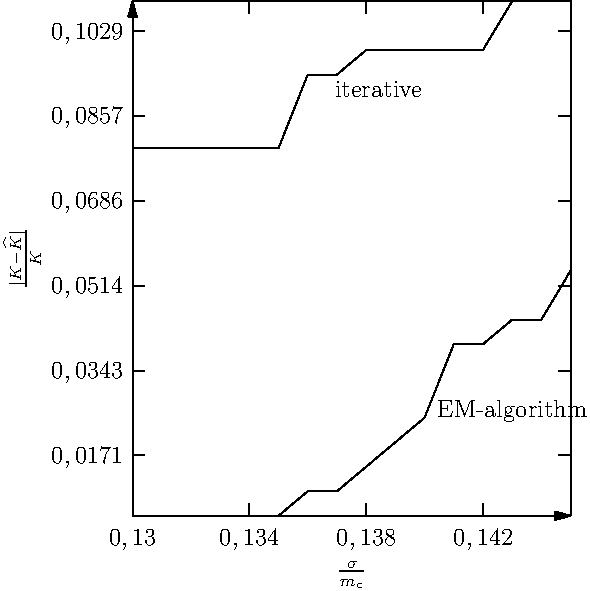
\includegraphics[height=7cm]{../../data/K_of_sigma.pdf}}
  \quad
  \subfloat[Зависимость относительной погрешности оценивания $|T_c|$ от $\sigma_c$.]%
{\label{fig:graph:lc0-Tc-sigma-c}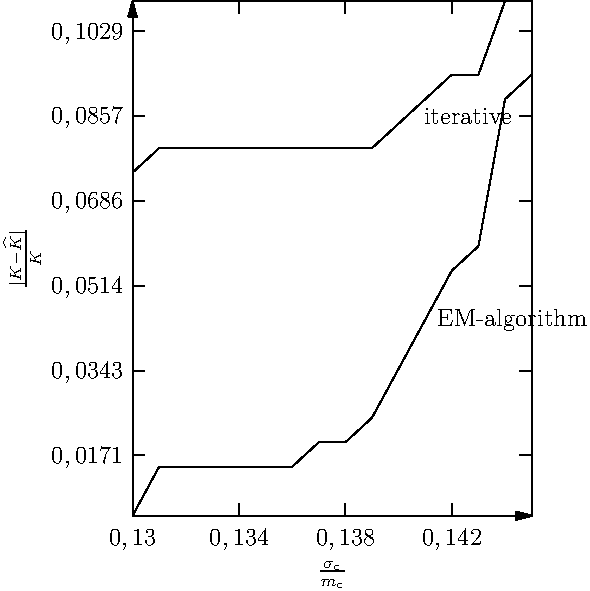
\includegraphics[height=7cm]{../../data/K_of_sigma_c.pdf}}
  \caption{Погрешности оценивания итеративным методом и EM-алгоритмом.}
  \label{fig:graph:lc0-Tc-errors}
\end{figure}

\subsection{Случай конечного времени обработки заявки}

%\appendix
%\section{Исходный код}
%\label{appendix:sources}

%\usestyle{default}

%\subsection{Title}
%\label{appendix:sources:sources-name}
%\includecode[python -O linenos=1]{data/source.py}

\pagebreak

\bibliographystyle{unsrt}
\bibliography{references}

\end{document}

% vim: set ts=2 sw=2 et:
